\noindent \texttt{V: 23-11-2019 11:35:00}

\section*{Experimento: - \textsc{Lei de Ampère}}
\section*{Teoria}
A Lei de Ampére fornece a integral do campo magnético $B$ em termos da intensidade de corrente elétrica: ela é proporcional à corrente líquida que atravessa a área limitada pelo caminho de integração $C$
\begin{comment}
\begin{equation}
   \oint _{C}{\mathbf  {B}}\cdot d{\mathbf  {l}}=\mu _{0}\int _{S}{\mathbf  {J}}\cdot d{\mathbf  {a}}=\int _{S}{\mathbf  {\nabla }}\times {\mathbf  {B}}\cdot d{\mathbf  {a}}\;.
\end{equation}
\end{comment}

\begin{equation}
    \oint _{C}{\mathbf  {B}}\cdot d{\mathbf  {l}}=\mu _{0}I
    \label{eq:eq-ampere-integral}
\end{equation}

\noindent 
Cabe ressaltar, que a Lei de Ampère é mais eficaz/útil para calcular os campos magnéticos criados por distribuições de corrente com \textbf{alto grau de simetria}, caso contrário é mais eficiente usar a Lei de Biot-Savart.

\noindent
Vamos analisar qual é o comportamento do campo magnético no centro de uma bobina. Sabe-se que uma carga elétrica em movimento ou uma corrente elétrica produz um campo magnético em sua vizinhança. Na Figura \ref{fig:bobina-lilith}, representa-se uma bobina de comprimento $L$, formada por $N$ espiras de seção reta circular de raio $r$. Uma corrente $I$ nas espiras produz um campo magnético $B$ cujo módulo, no centro da bobina, é dado por:
\begin{equation}
    \mathbf{B}=\frac{\mu\,\mathbf{I}N}{L}\cos \alpha\;,
\end{equation}

\noindent
em que $\mu$ é a permeabilidade magnética do meio no interior da bobina e $\cos \alpha$ é um fator de
correção do campo, introduzido pelo fato de o comprimento da bobina ser finito (veja Figura \ref{fig:bobina-lilith}). A
permeabilidade magnética para o ar é $\mu_{ar} \cong \mu_{0} = 1,26 \times 10^{-6}\,Tm/A$. 
A direção desse campo é ao longo do eixo da bobina e seu sentido é dado pela "regra da mão direita" (\textbf{Lei de Ampère}).

\begin{wrapfigure}{r}{0.7\textwidth}
    \centering
    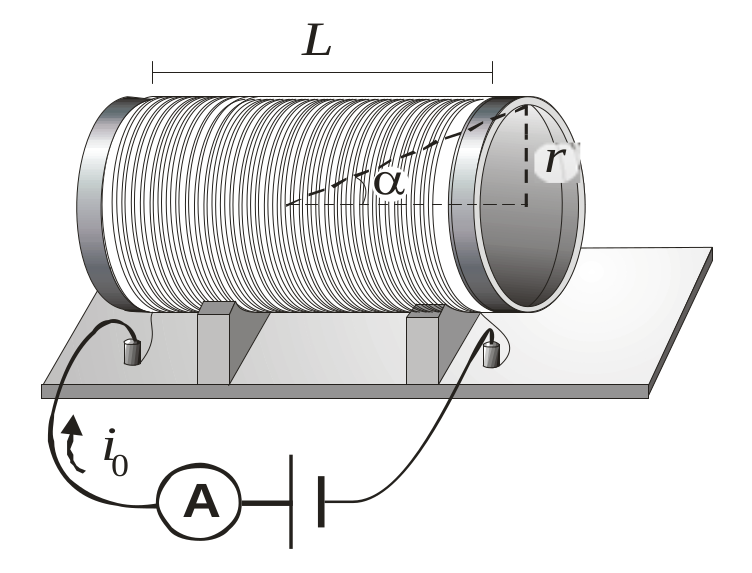
\includegraphics[width=.36\textwidth]{img/bobina-lilith.png}
    \caption{Bobina cilíndrica de comprimento L e de raio r, ligada a uma fonte de
corrente elétrica, que produz um campo magnético em seu interior. \textit{Fonte: \href{http://lilith.fisica.ufmg.br}{lilith.fisica.ufmg.br}}.}
    \label{fig:bobina-lilith}
\end{wrapfigure}

\noindent

Sabe-se que a força que um campo magnético $B$ exerce sobre um fio reto que transporta uma
corrente elétrica $I$ é dada por

\begin{equation}
    \mathbf{F}=\mathbf{I}\,l\times \mathbf{B}\;,
\end{equation}

\noindent 
em que {\color{red}$l$ é um \textbf{vetor} dirigido ao longo do fio}, no sentido da corrente elétrica, com módulo igual ao
comprimento do fio.

\noindent
O módulo do campo magnético em uma certa região pode ser determinado por meio da
medição dessa força. E a direção pode ser determinada usando uma bússola.

\section*{Prática}

	\section{Objetivos}
	
\noindent 
Comprovar experimentalmente a existência e forma das linhas de campo gerados por condutores percorridos por corrente elétrica demonstrando a Lei de Ampère e observar o comportamento da força magnética entre dois fios paralelos conduzindo correntes elétricas em dois cenários, a saber, no mesmo sentido e no sentido contrário.

	\section{Material utilizado}
	
	\begin{itemize}
		\item[a)] Fonte de Tensão e Corrente (Min $15\,A$) Contínua (CC);
		\item[b)] Fios ou cabos ou fitas condutoras;
		\item[c)] Um multímetro;
		\item[d)] Fios ou cabos condutores com terminais "banana" ou "jacaré" para uso geral;
		
	\end{itemize}

	\section{Procedimento experimental}
	
	\subsection*{A - Campo gerado por corrente elétrica em um solenóide}
	Montar o experimento seguindo a instrução do professor;
	
	\begin{equation}
    \mathbf{B}=\frac{\mu\,\mathbf{I}N}{L}\cos \alpha\;,
\end{equation}
	
	\subsection*{B - Força elétrica entre condutores paralelos}
	Montar o experimento seguindo a instrução do professor;
	
	\begin{equation}
    \mathbf{F}=\mathbf{I}\,l\times \mathbf{B}\;,
\end{equation}

\section{Relatório ou Exercícios}

\begin{itemize}
\item Construa o relatório apresentando os itens obrigatórios; 
\item Comente as prováveis fontes de erro;
\item Responda as questões formuladas;
\item Apresente os dados organizados em tabelas; 
\item Apresente a análise dos dados e gráficos; 
\item Apresente os resultados solicitados no Sistema Internacional de unidades com todos os cálculos efetuados.
\end{itemize}

\noindent
{\color{red} \rule{\linewidth}{0.5mm} }
\textbf{Dica:}

\noindent \texttt{ O que se espera? Algo do tipo...}

\begin{figure}[H]
	\centering
	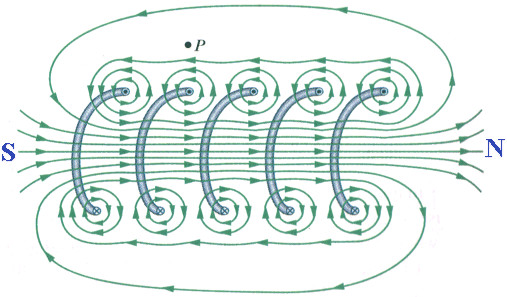
\includegraphics[scale=.5]{img/solenoide1.jpg}
	\caption{Campo magnético gerados por correntes elétricas em solenoides. \textit{Fonte: \href{http://ensinoadistancia.pro.br/EaD/Eletromagnetismo/LeiAmpereExe/LeiAmpereExe.html}{UNB}}.}
	\label{fig:fig-campo-solenoide}
\end{figure}

\begin{figure}[H]
	\centering
	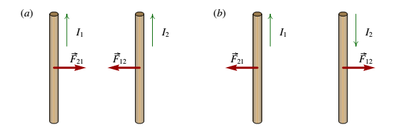
\includegraphics[scale=.7]{img/forcas-magneticas_entre_dois_fios_com_corrente.png}
	\caption{Força entre condutores com corrente. \textit{Fonte: \href{https://pt.wikipedia.org/wiki/For\%C3\%A7a_magn\%C3\%A9tica}{Wikipedia}}.}
	\label{fig:fig-forca-condutores-paralelos}
\end{figure}